\documentclass[Bachelorarbeit.tex]{subfiles}
\begin{document}

\graphicspath{{./figures/newMarket/}}	%specifying the folder for the figures

\chapter{A new Market}
As already introduced in chapter \ref{ch:interpretation} "Interpretation" a new market in which agents can trade collateralized assets against cash is necessary to elevate the miss-allocation of collateralized assets in the range of the pessimist agents.

\section{Implementation}

\subsection{Price-Range}
min, max, limit price

min = Math.min( 0, this.minAssetPriceInCash - this.maxLoanPriceInCash );
max = this.maxAssetPriceInCash - this.minLoanPriceInCash;
limit = this.limitPriceCollateral = this.limitPriceAsset - this.limitPriceLoan;\\

\subsection{Bid-Offering}
can make offering only when cash greater epsilon
give asset-price in cash formula
give asset-amount formula
	
\subsection{Ask-Offering}
can make offering only when there are collateralized assets: currentObligations greater epsilon
give asset-price in cash-formula
give asset-amount formula

\subsection{Sell-Match}
Verkäufer: 	bekommt Cash und gibt Asset und Loan

\subsection{Buy-Match}
Käufer: bekommt Asset und Loan, zahlt Cash

\section{Results with the new market}	
As experiment-configuration the same as given in Chapter  "Results" is used.

\begin{table}[h]
	\centering
	\caption{Configuration for all experiments}
	\begin{tabular} { l c r }
		\hline
		Agent-Count & 100 \\
		Bond-Type & 0.5 \\
		Replication-Count & 50 \\
		Terminate after & 1000 failed successive Transactions \\
		\hline
	\end{tabular}
\end{table}

\begin{figure}[H]
	\centering
  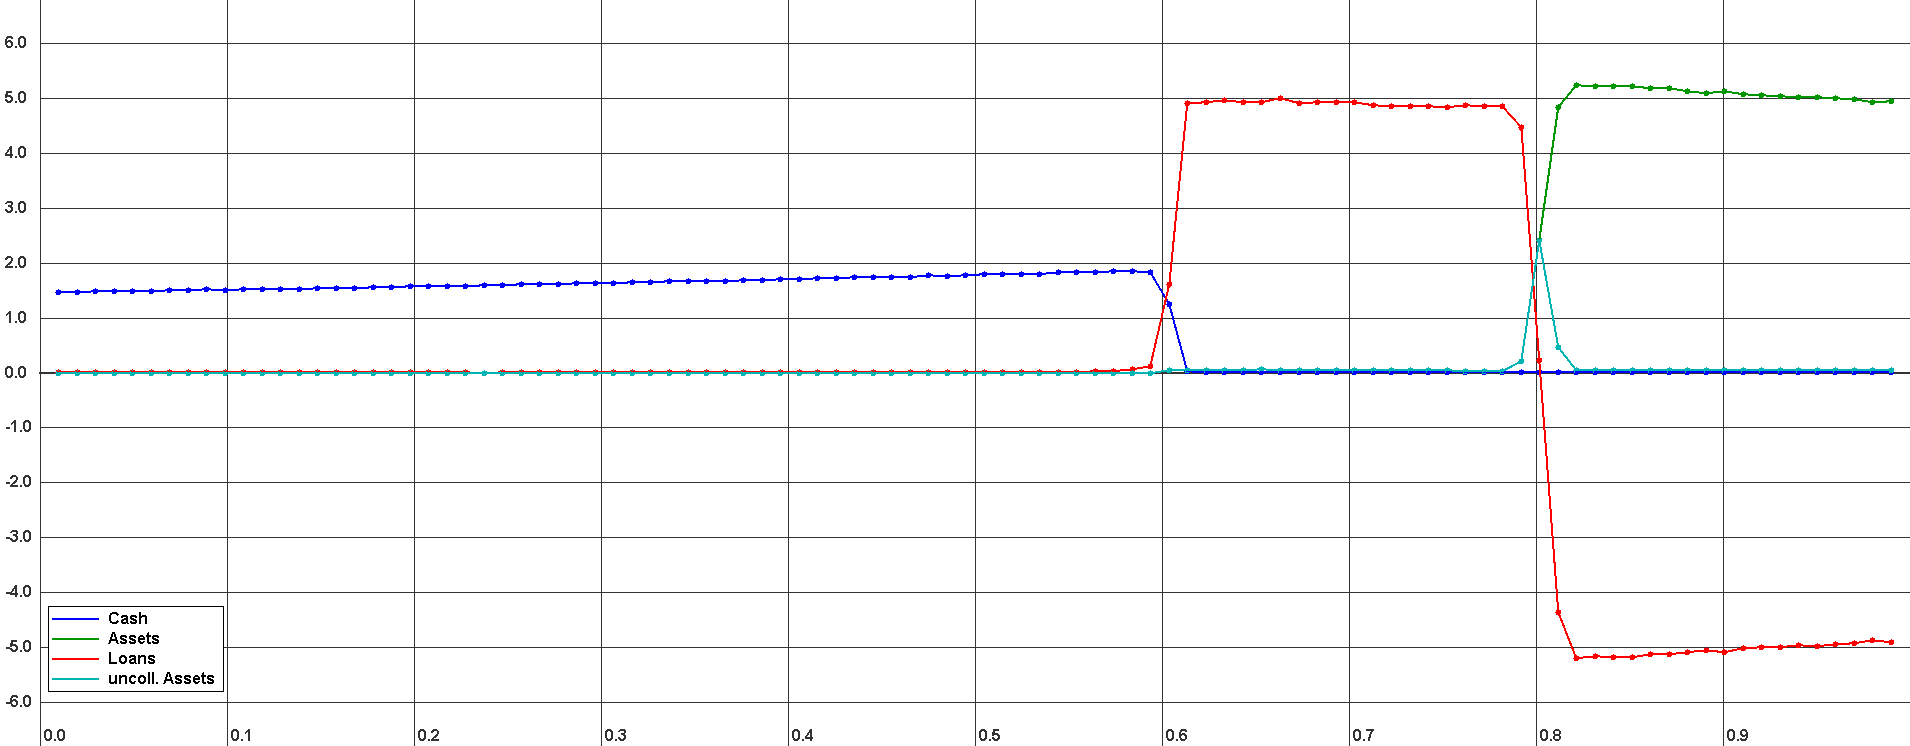
\includegraphics[width=1.0\textwidth, angle=0]{FULLYCONNECTED_100_WITHCOLLATERALMARKET_REPL.png}
	\caption{Wealth-Distribution of Fully-Connected topology with collateral/cash market}
	\label{fig:wealth_FULLYCONNECTED_100_WITHCOLLATERALMARKET_REPL}
\end{figure}

\begin{table}[h]
	\caption{Equilibrium of Fully-Connected topology with collateral/cash market}
	\centering
	\begin{tabular} { l c r }
		\hline
		Asset-Price & 0.688 (0.008) \\
		Loan-Price & 0.381 (0.002) \\
		i0 (Marginal Buyer) & 0.597 (0.005) \\
		i1 (Marginal Seller) & 0.803 (0.003) \\
		Pessimist Wealth & 1.597 (0.009) \\
		Medianist Wealth & 4.76 (0.1) \\
		Optimist Wealth & 4.963 (0.052) \\
		\hline
	\end{tabular}
\end{table} 

\begin{table}[h]
	\caption{Performance of Fully-Connected topology with collateral/cash market}
	\centering
	\begin{tabular} { l c r }
		\hline
		Successful TX & 1916.14 (31.42) \\
		Total TX & 6364.8 (1679.21) \\
		Failed TX & 4448.66 (1668.93) \\
		\hline
	\end{tabular}
\end{table}

\begin{figure}[H]
	\centering
  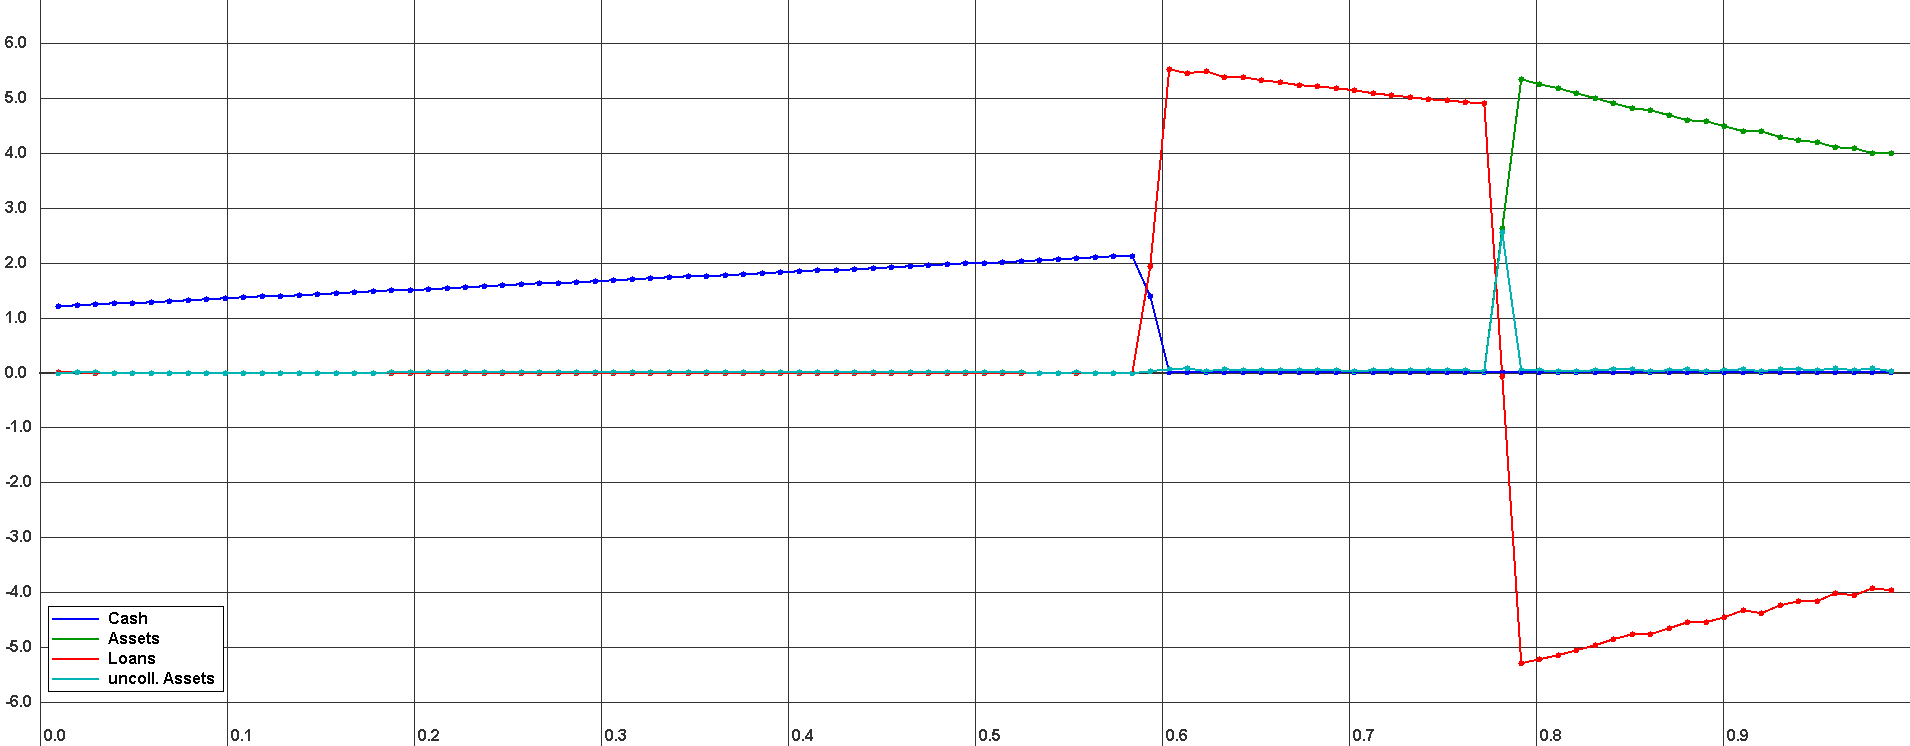
\includegraphics[width=1.0\textwidth, angle=0]{ASCENDINGCONNECTED_100_WITHCOLLATERALMARKET_REPL.png}
	\caption{Wealth-Distribution of Ascending-Connected topology with collateral/cash market}
	\label{fig:wealth_ASCENDINGCONNECTED_100_WITHCOLLATERALMARKET_REPL}
\end{figure}

\begin{table}[h]
	\caption{Equilibrium of Ascending-Connected topology}
	\centering
	\begin{tabular} { l c r }
		\hline
		Asset-Price & 0.713 (0.013) \\
		Loan-Price & 0.383 (0.005) \\
		i0 (Marginal Buyer) & 0.584(0.0) \\
		i1 (Marginal Seller) & 0.782 (0.0) \\
		Pessimist Wealth & 1.671 (0.0) \\
		Medianist Wealth & 5.032 (0.013) \\
		Optimist Wealth & 4.508 (0.006) \\
		\hline
	\end{tabular}
\end{table} 

\begin{table}[h]
	\caption{Performance of Ascending-Connected topology}
	\centering
	\begin{tabular} { l c r }
		\hline
		Successful TX & 51,838.74 (1613.36) \\
		Total TX & 52.963.5 (1612.31) \\
		Failed TX & 1124.76 (28.31) \\
		\hline
	\end{tabular}
\end{table}

TODO: difference to theoretical equilibrium

\section{Market dynamics}
In the thesis-software it is possible to run an ascending-connected topology until no more trades are possible and then activate the new market. the collateralized assets are bought and sold by the pessimists and move up the optimism-scale until they end up in the optimists.

\begin{figure}[H]
	\centering
  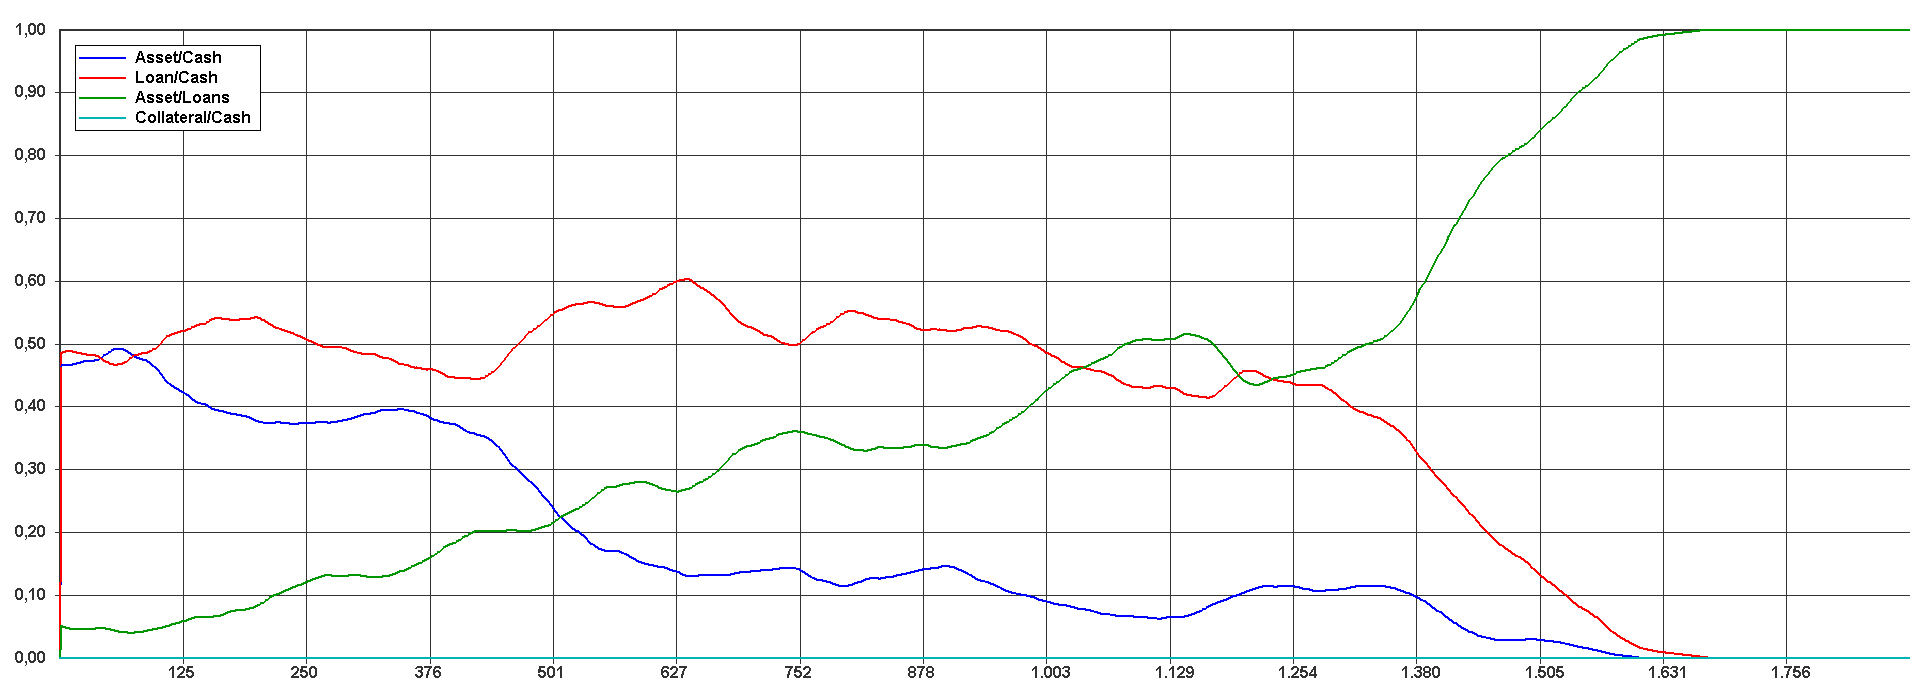
\includegraphics[width=1.0\textwidth, angle=0]{FULLYCONNECTED_100_NOCOLLATERALMARKET_MARKETSTIME_SINGLE.png}
  	\caption{Market-activity over time of Fully-Connected topology without collateral/cash market}
	\label{fig:wealth_FULLYCONNECTED_100_WITHCOLLATERALMARKET_MARKETSTIME_REPL}
\end{figure}

\begin{figure}[H]
	\centering
  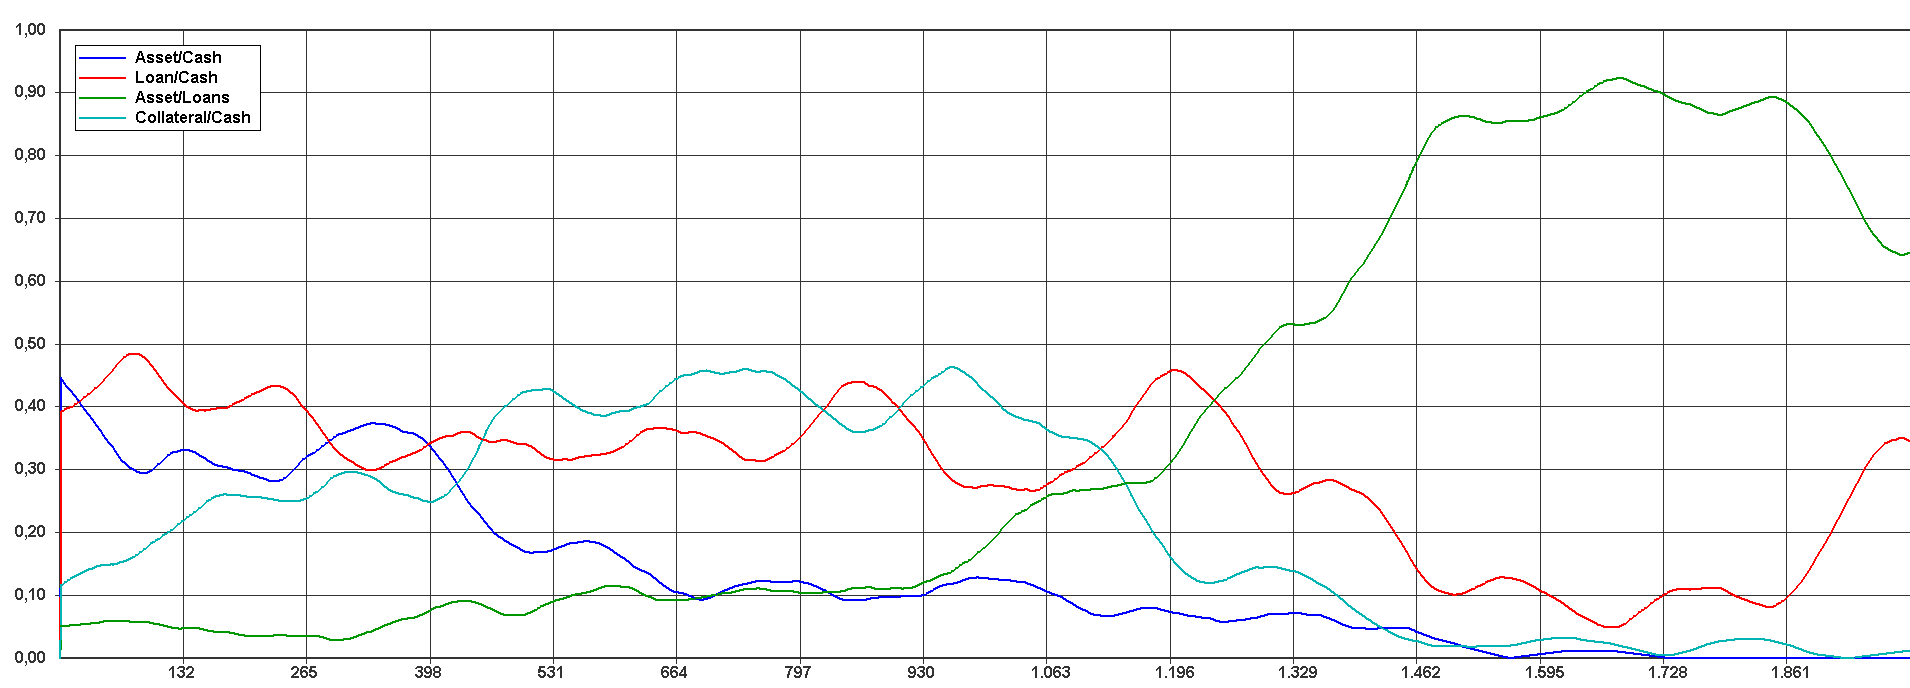
\includegraphics[width=1.0\textwidth, angle=0]{FULLYCONNECTED_100_WITHCOLLATERALMARKET_MARKETSTIME_SINGLE.png}
  	\caption{Market-activity over time of Fully-Connected topology with collateral/cash market}
	\label{fig:wealth_FULLYCONNECTED_100_WITHCOLLATERALMARKET_MARKETSTIME_REPL}
\end{figure}


\begin{figure}[H]
	\centering
  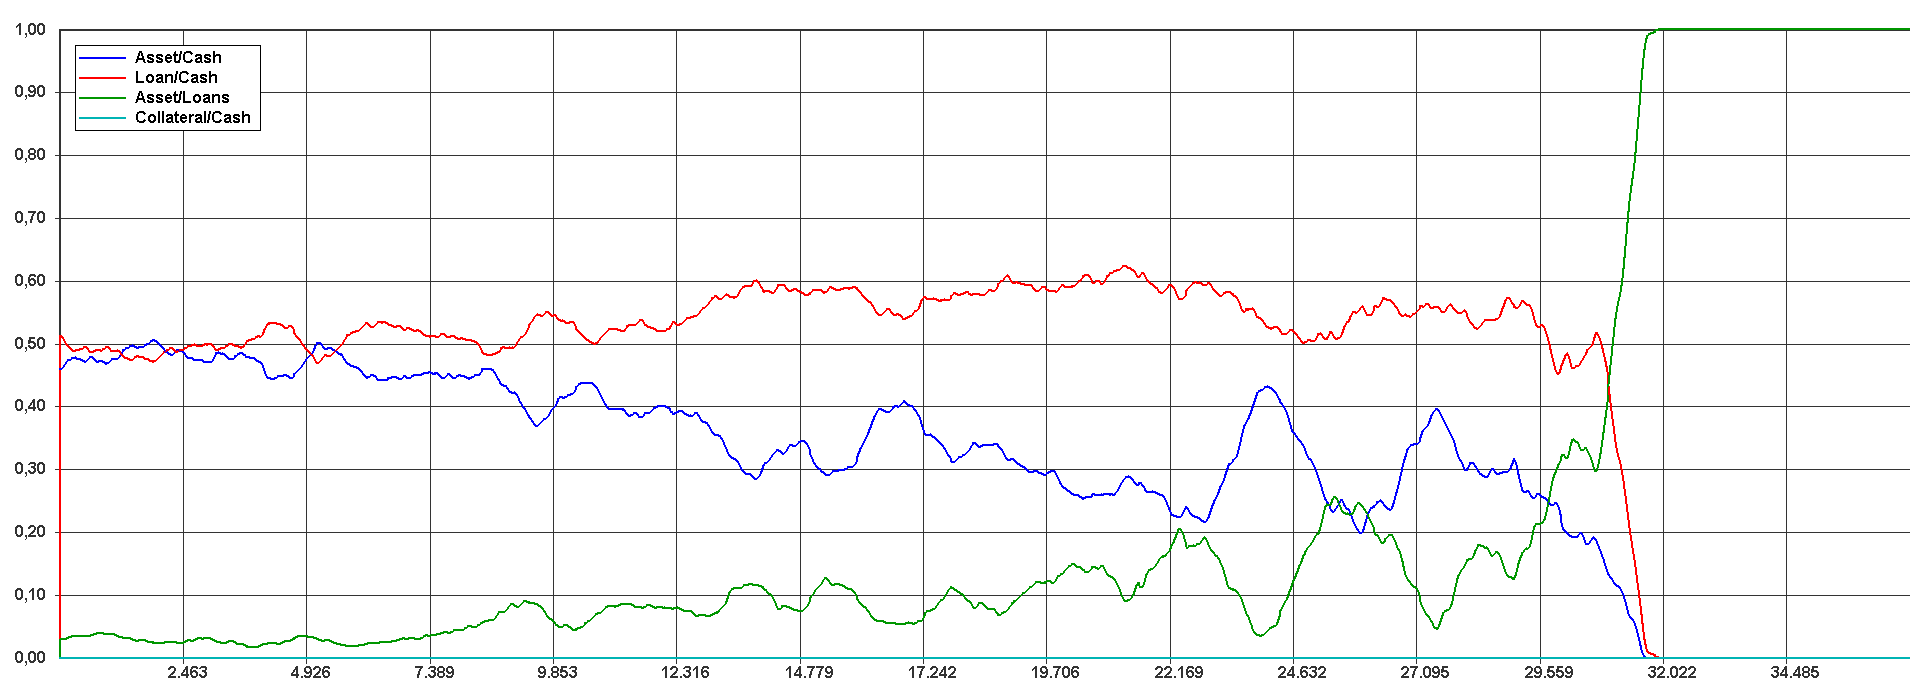
\includegraphics[width=1.0\textwidth, angle=0]{ASCENDINGCONNECTED_100_NOCOLLATERALMARKET_MARKETSTIME_SINGLE.png}
	\caption{Market-activity over time of Ascending-Connected topology without collateral/cash market}
	\label{fig:wealth_ASCENDINGCONNECTED_100_WITHCOLLATERALMARKET_MARKETSTIME_REPL}
\end{figure}

\begin{figure}[H]
	\centering
  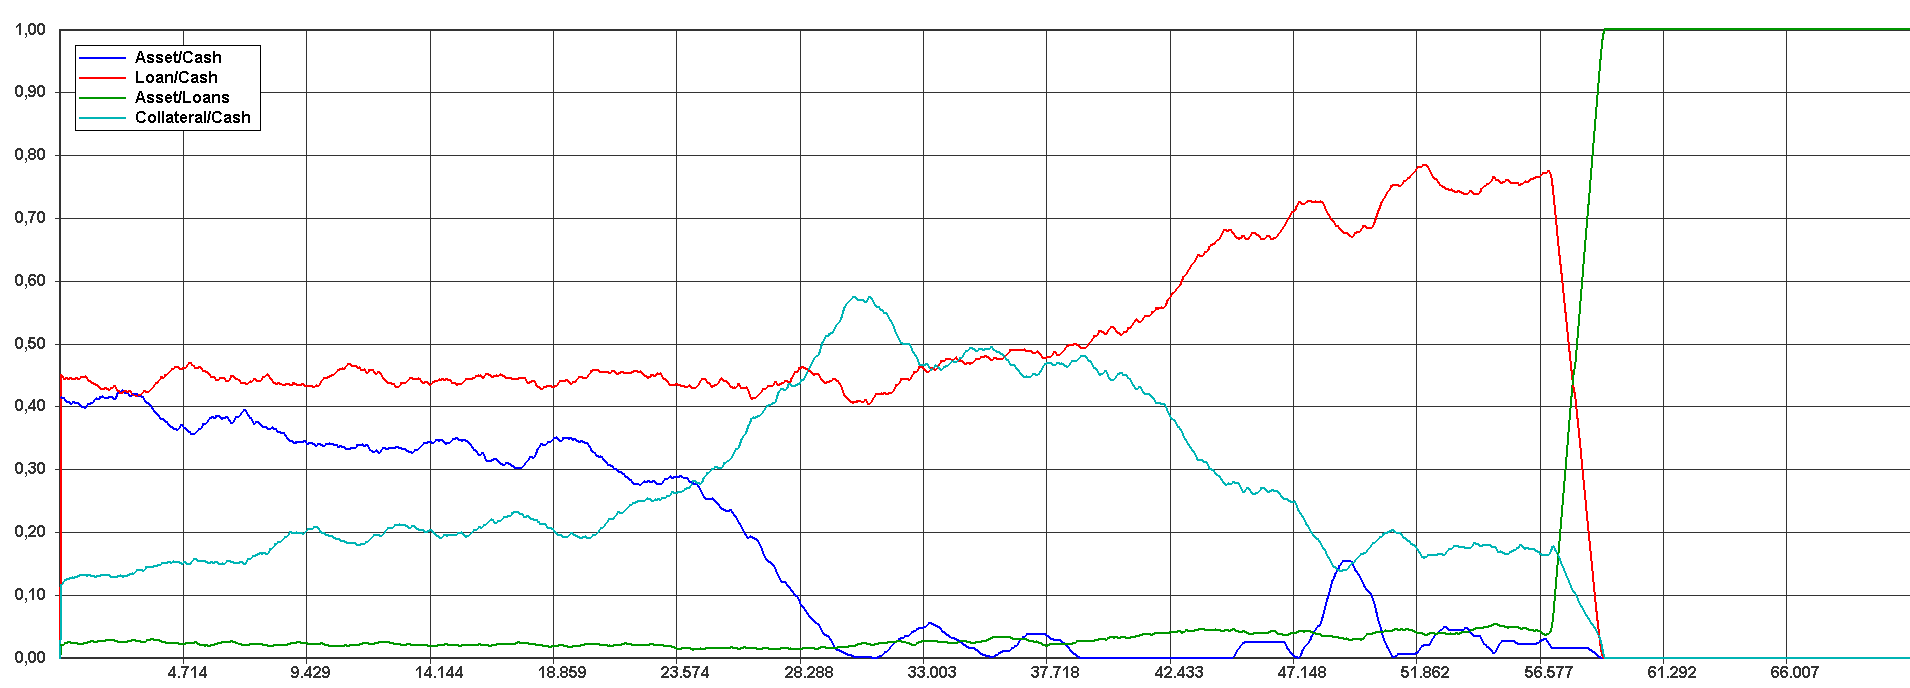
\includegraphics[width=1.0\textwidth, angle=0]{ASCENDINGCONNECTED_100_WITHCOLLATERALMARKET_MARKETSTIME_SINGLE.png}
	\caption{Market-activity over time of Ascending-Connected topology with collateral/cash market}
	\label{fig:wealth_ASCENDINGCONNECTED_100_WITHCOLLATERALMARKET_MARKETSACCUM_REPL}
\end{figure}

\begin{figure}[H]
	\centering
  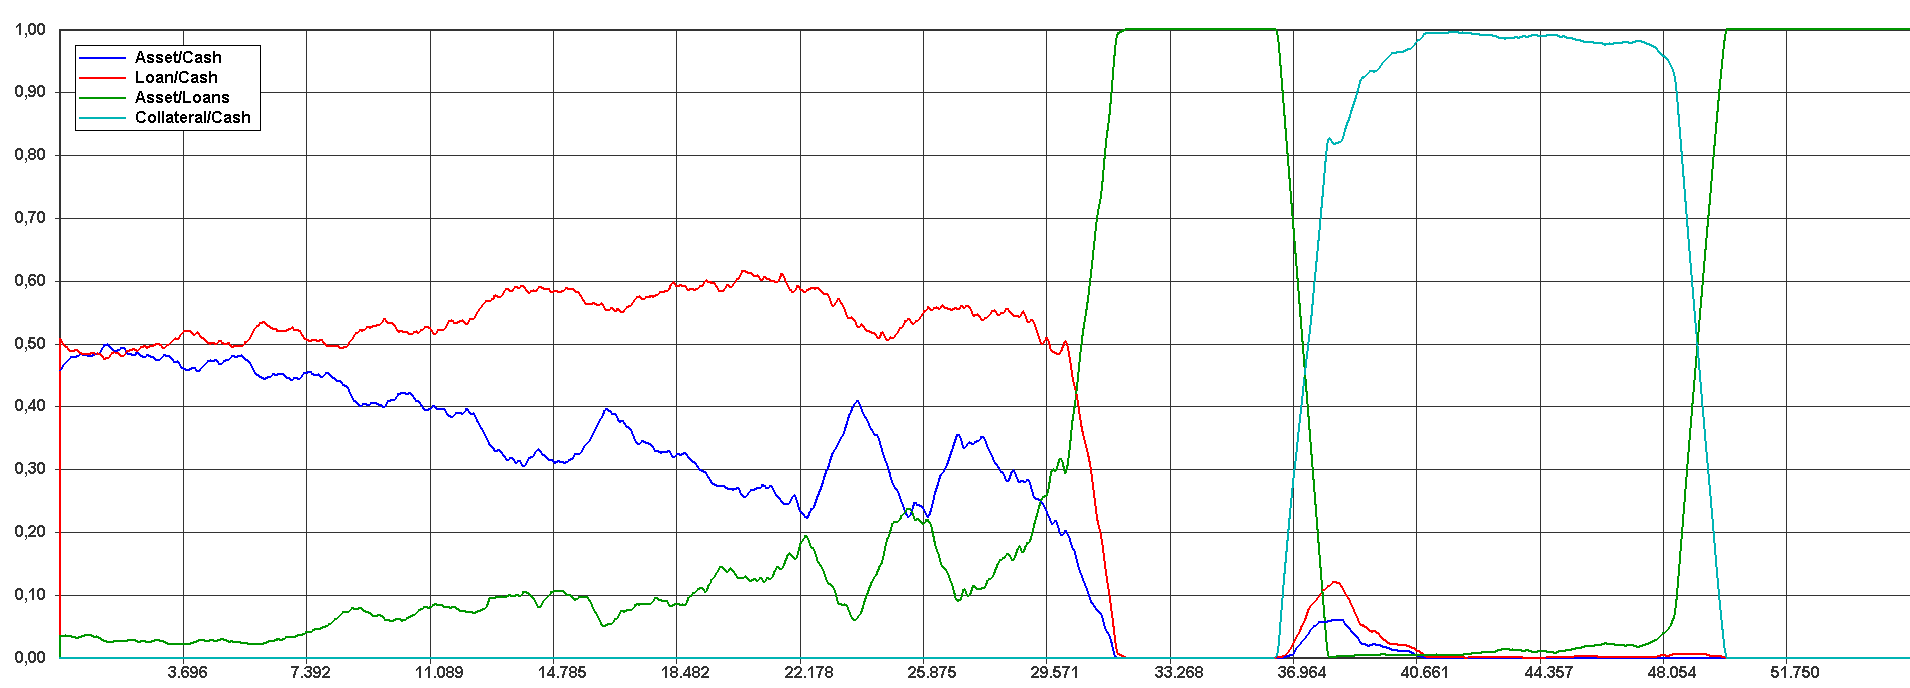
\includegraphics[width=1.0\textwidth, angle=0]{ASCENDINGCONNECTED_100_WITHCOLLATERALMARKET_DEFERREDACTIVATION_MARKETSTIME_SINGLE.png}
	\caption{Market-activity over time of Ascending-Connected topology with collateral/cash market activated only after 1000 failed transactions in a row. Previous dynamics the same as figure \ref{fig:wealth_ASCENDINGCONNECTED_100_WITHCOLLATERALMARKET_MARKETSTIME_REPL}}
	\label{fig:wealth_ASCENDINGCONNECTED_100_WITHCOLLATERALMARKET_DEFERREDACTIVATION_MARKETSTIME_SINGLE}
\end{figure}

\section{Interpretation of new Market}
the equilibrium is different than the fully-connected one thus the hypothesis is still wrong.
rooted in the fundamental different trading dynamics in ascending-connected compared to fully-connected as can be seen in the market-dynamics

TODO: wie passiert schlussendlich das unkollateralisieren von assets? die kollateralisierten assets werden ja nicht unkollateralisiert sondern wandern einfach zu den optimisten. unkollateralisiert werden sie ja nicht. die medianisten haben keinen cash mehr und kaufen assets gegen bonds und unkollateralisieren sie. genau erklären.


\end{document}
